% !TEX root = ../thesis.tex

\chapter{Experiment Setup}

The experiment is divided into three parts in order to address the three research questions proposed in Section 1.2. In this chapter, everything needed to conduct the experiment, such as the dataset, system specifications, hyperparameter selection, etc., is described in seven sections. The section \textit{Clustering evaluation} details the evaluation of clustering results and the selection of the best parameters for the proposed pipeline. Subsequently, the section \textit{Survey evaluation} illustrates the survey design, \ac{IR} system introduction, and comparison strategy. Finally, the section \textit{Precision evaluation} introduces the literature comparison and retrieval performance strategies.



	\section{System Specifications}

The experiment is carried out in two different systems according to the time taken to execute specific tasks. All the code development, exploratory analysis, and statistical testing are performed on an HP ELITEBOOK system with an AMD Ryzen 5 PRO 4650U processor, 16 GB of RAM, and 500 GB of disk space. Web scraping, \ac{IR} system hosting, data storage, clustering, and further benchmark testing are performed on a large \ac{VM} hosted at \ac{FKIE}. The technical specifications of the \ac{VM} are four processors CPU (Intel(R) Xeon(R) Gold 6136 CPU @ 3.00GHz), 48 GB RAM, and 370 GB disk space.
	
	
	\section{Testset Description}

For two main reasons, finding a dataset specific to this research problem is difficult in the current \ac{IR} data repositories. Firstly, the search query needs to be a phrase rather than a sentence. Furthermore, the documents need to be labeled with a specific intention rather than just coherence with the query. The interest at \ac{FKIE} is to retrieve the documents related to "Innovation and Technology," and a new test set is collected for this purpose. Below are a few specific areas of interest in news articles that describe the user intention: \textit{Innovation, Technology breakthroughs, Future products, Applied research, New procurement strategies,} and \textit{Artificial Intelligence}. These topics are also described as positive document characteristics because a document is considered positive when it is strongly related to any of the above-mentioned characteristics.


The strategy for test set collection is to consider documents from lexical and semantic matching. The results from both algorithms help find the diverse contexts related to the user query. Therefore, a candidate pool with a maximum length of 30 documents is considered. Fifteen lexical and semantic matching documents are combined into a merged set where duplicate documents are removed. Relevance labeling is the task of assigning an appropriate label to the retrieval results inside the candidate pool by multiple independent labelers. Every labeler has to assign a label coherent with the query and consider the \ac{FKIE} user's intention, i.e., coherence with the positive document characteristics mentioned above. Once the labeler assigns a particular label to a document, the labeled information is stored in an SQLite DB.


\mycomment{

\begin{figure}[h]
	\centering
	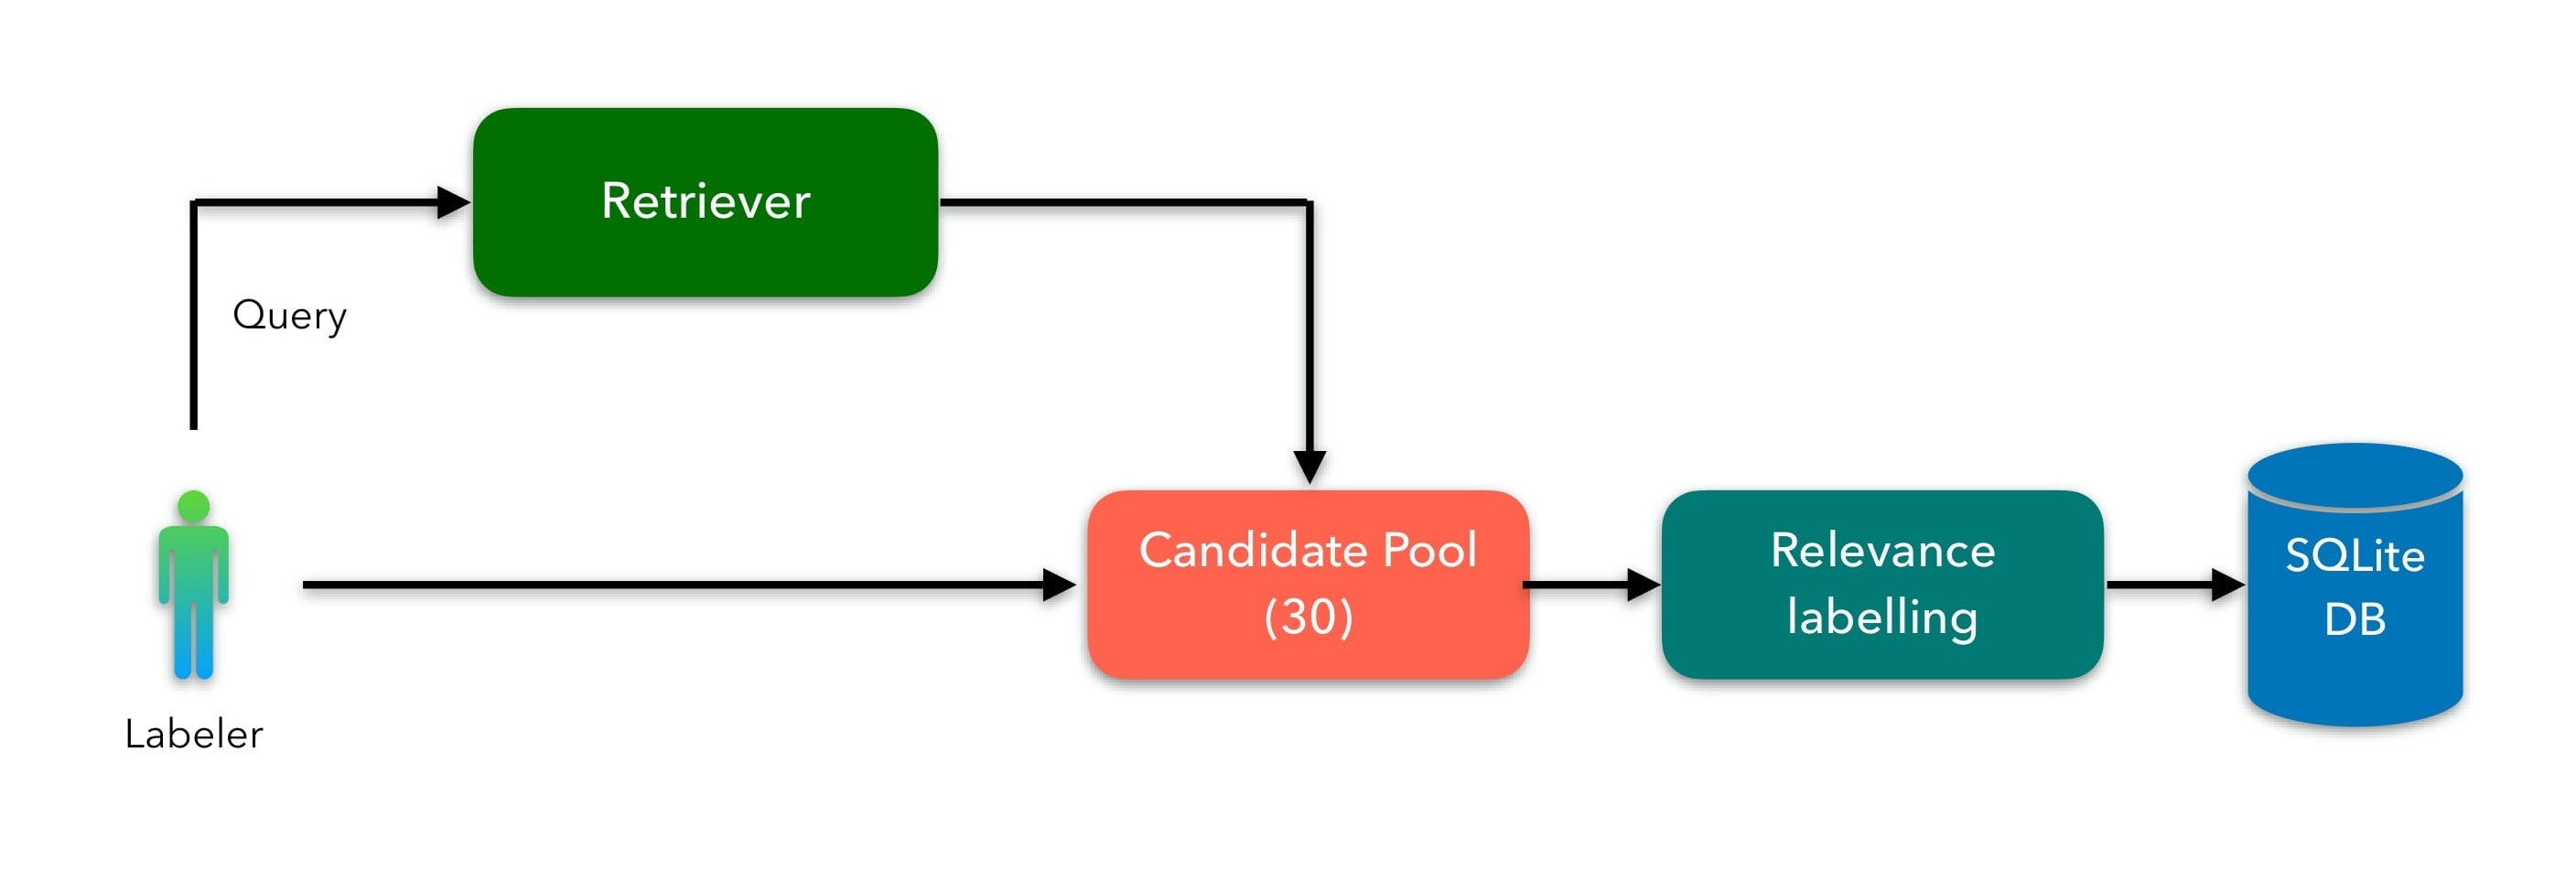
\includegraphics[width=.8\textwidth]{images/keynotes_images/dataset.jpg}
	\caption{Testset collection strategy. \label{fig:dataset}}
\end{figure}
}

\begin{center}
	\captionof{table}[Relevance labels introduction and details.]{Relevance labels definition and document distribution.}\label{tab:label_definitions}
	\begin{tabularx}{0.85\textwidth}{|c|c|c|Y|}
		\hline
		Label-id & Label name & Document count &  Label definition  \\
		\hline
		1 & Perfect & 78 &A document that strongly matches  one of the positive document characteristics. \\
		\hline
		2 & Partially relevant & 147 &  A document that contains keywords and seems to be relevant, but still lacks innovation or novelty. \\
		\hline
		3 & Irrelevant & 306 & A document containing the given user keyword still lacks innovation and
		coherent discussion about the query. Eg: click-baits, advertisements, etc,. \\
		\hline
		4 & Wrong & 98 & These are false documents and have nothing to do with the user	query. \\
		\hline
	\end{tabularx}
\end{center}

A total of 22 queries are labeled by 5 different labelers. After analyzing the label distribution of the queries, it is observed that the distributions of perfect and partially relevant documents are very low compared to the other labels, as shown in \prettyref{tab:label_definitions}. For evaluation, 17 queries are considered. The queries and their respective label details are shown in \prettyref{tab:testset_queries}.

\begin{center}
	\captionof{table}{Testset queries used for the evaluation.}\label{tab:testset_queries}
\begin{tabularx}{0.95\textwidth}{|c|c|Y|Y|Y|Y|}
	\hline
	S No. & Query & Perfect & Partially relevant & Irrelevant & Wrong \\
	\hline
1	&  Architekturanalyse & 4 & 6 & 15 & 4 \\
	\hline
2	& Big Data, KI für Analyse	 & 7 & 11 & 10 & 2 \\
	\hline
3	& Edge computing & 1 & 5 & 11 & 11 \\
	\hline
4	& IT-Standards & 1 & 7 & 9 & 11 \\
	\hline
5	&  Kommunikationsnetze & 4 & 5 & 18 & 1 \\
	\hline
6	& Methode Architektur & 4 & 8 &  15 & 2 \\
	\hline
7	& Militärische Kommunikation & 7 & 5 & 18 & 0 \\
	\hline
8	& Mixed Reality	 & 5 & 10 & 8  & 6 \\
	\hline
9	& Quantentechnologie & 3 & 4 & 16 & 1 \\
	\hline
10	& Robotik & 15 & 8 & 6 & 0 \\
	\hline
11	& Satellitenkommunikation & 2 & 6 & 21 & 1 \\
	\hline
12	& Schutz von unbemannten Systemen & 7 & 11 & 12 & 0 \\
	\hline
13	& Visualisierung  & 5 & 4 & 10  & 11 \\
	\hline
14	& Waffen Systeme & 6 & 15 & 8 &  0\\
	\hline
15	& Wellenformen und -ausbreitung	 & 4 & 13  & 8 &  5\\
	\hline
16	& militärische Entscheidungsfindung	 & 1 & 6 & 20 & 3 \\
	\hline
17	& unbemannte Landsysteme & 2 & 10 & 1 & 17 \\
	\hline

\end{tabularx}
\end{center}


Five queries are removed from this test set due to either no perfect documents or very few perfect and partially relevant documents. These queries are considered outliers and can lead to incorrect results in the target function. The removed queries, along with their label distribution, are shared in \prettyref{tab:removed_queries}. The final data collected through the labeling process is published in the GitHub repository \textit{Thesis-retrieval-data}\footnote{\url{https://github.com/praveengadiyaram369/Thesis-retrieval-data}}.


\begin{center}
	\captionof{table}{Queries removed from the testset.}\label{tab:removed_queries}
	\begin{tabularx}{0.95\textwidth}{|c|c|Y|Y|Y|Y|}
		\hline
		S No. & Query & Perfect & Partially relevant & Irrelevant & Wrong \\
		\hline
		1	&  Kryptologie & \textbf{0} & 0 & 4 & 14 \\
		\hline
		2	& Defense	 & \textbf{0} & 1 & 29 & 0 \\
		\hline
		3	& Cyber Attack & \textbf{0} & 2 & 27 & 0 \\
		\hline
		4	& Data Centric Warfare & \textbf{0} & 4 & 21 & 5 \\
		\hline
		5	&  unbemannte Wirksysteme & \textbf{0} & 6 & 19 & 4 \\
		\hline
	
		
	\end{tabularx}
\end{center}


\mycomment{\begin{center}
		\captionof{table}{Label distributions in the testset.}\label{tab:label_distribution}
		\begin{tabularx}{0.6\textwidth}{|c|Y|c|}
			\hline
			Label-id & Label name & Document count \\
			\hline
			1 & Perfect & 78 \\
			\hline
			2 & Partially relevant & 147 \\
			\hline
			3 & Irrelevant & 306 \\
			\hline
			4 & Wrong & 98 \\
			\hline
		\end{tabularx}
\end{center}}

\section{Preprocessing for Efficient Retrieval}

As described in Section 2.3, the setup of the \ac{IR} system involves web scraping news articles, filtering out articles unrelated to technology and the military, and storing the articles in two separate document indices to facilitate information retrieval. Sub-topic modeling is performed on this \ac{IR} setup to extract a candidate pool and select candidate keywords, which are crucial steps in generating diverse sub-topics. Both steps utilize a \ac{USE} model to encode the documents and keywords into distributed semantic embeddings.


\begin{figure}[h]
	\centering
	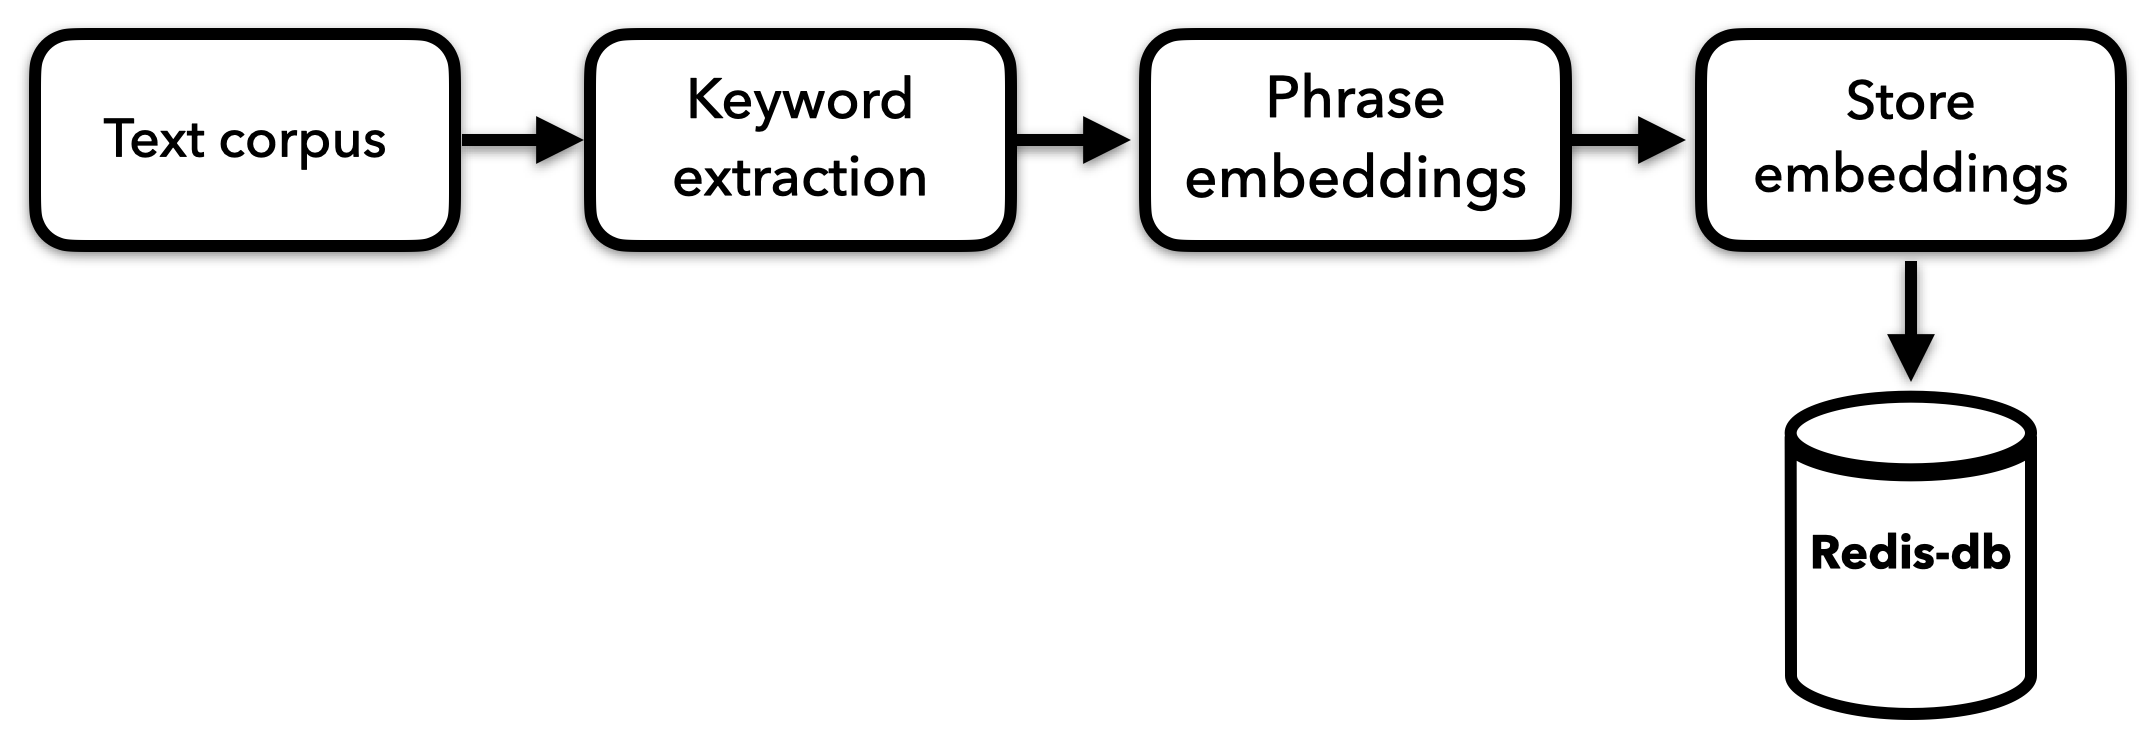
\includegraphics[width=.9\textwidth]{images/thesis_images/redisdb.png}
	\caption[Pjpeline for efficient sub-topics.]{Preprocessing pipeline for efficient sub-topic modeling. \label{fig:redis_db}}
\end{figure}

Manual analysis of sub-topic modeling reveals that the encoding time for a text using a \ac{USE} model is high. This results in users having to wait for a response from the \ac{IR} system. To overcome this, a cache system is developed to store the keyword embeddings obtained from the \ac{USE} model in a Redis-DB. \prettyref{fig:redis_db} illustrates the pipeline implemented to improve the time required for sub-topic modeling and clustering. The performance of sub-topic retrieval using the cache is evaluated against retrieval without using the cache. The mean time taken in seconds for sub-topic retrieval across 28 search queries is considered as the evaluation metric. Let us denote the time taken for retrieving sub-topics for one query $q$ as $t_q$, and the mean time over $N$ queries as $Mt$.


\centerline{$Mt$ = ($\sum\limits_{i=1}^N t_i) /N$}

The lower the time taken to retrieve sub-topics, the more efficient the approach is considered. \prettyref{tab:cache_comparision} provides a comparison of the mean time taken in seconds for the two approaches. It is observed that caching keyword embeddings results in sub-topic retrieval that is almost 10 times faster, making it a more efficient approach. Sub-topic retrieval without caching the keywords can take up to one minute, which can negatively impact the usability of this proposed candidate keyword selection approach in real-time.


\begin{center}
	\captionof{table}[Performance comparison of caching.]{Performance comparison of caching keyword embeddings.}\label{tab:cache_comparision}
	\begin{tabularx}{0.77\textwidth}{|Y|Y|}
		\hline
		 Sub-topic retrieval approach &  Mean time taken in seconds ($Mt$) \\
		\hline
	 With caching & \textbf{7.75} \\
		\hline
	 Without caching & 77.41 \\
		\hline
	\end{tabularx}
\end{center}


\section{Clustering Evaluation}

The main objective of this evaluation is to determine the parameters of the sub-topic modeling that create clusters representing the candidate pool in the best and most diverse manner. Since there are no cluster labels available for the queries in the test set, an alternative approach is adopted to assess the quality of the generated clusters.

	
	\subsection{Intrinsic Evaluation:} In the case of no labeled data, the clustering output is generally evaluated using an intrinsic evaluation approach. The Silhouette index is a metric used for evaluating the clustering performance and is calculated by using the intra-cluster and inter-cluster distances for each sample~\cite{rousseeuw1987silhouettes, shutaywi2021silhouette}. Let us consider the test set $T$ as a set of data points where each data point is denoted as $x_i$.
		
		\centerline{$T$ = $\{x_1, x_2, x_2,\dots\}$}
		
		The testset $T$ is clustered using a clustering algorithm resulting the data points segregated into groups. Let us consider the cluster set $C$ where each cluster is denoted as $c_i$.
		
		\centerline{$C$ = $\{c_1, c_2, c_2,\dots\}$}
		
		The silhouette index $s(x_i)$ for a data point $x_i$ which is an element of cluster $c_k$ is expressed as below.\\
		
		\centerline{$s(x_i)$ = $\frac{b(x_i) - a(x_i)}{max(b(x_i), a(x_i))} $}
		
The value $a(x_i)$ represents the mean distance between the data point $x_i$ and all other data points inside the cluster $c_k$. On the other hand, $b(x_i)$ represents the mean distance between the data point $x_i$ and all other data points in the nearest cluster $c_l$~\cite{shutaywi2021silhouette}. These values, $a(x_i)$ and $b(x_i)$, respectively represent the intra-cluster and inter-cluster distances. The silhouette score $s(x_i)$ is calculated for all the data points in the test set, and the final mean is considered as the silhouette score $S$ of the clustering. The silhouette score ranges from -1 to 1, with a higher score representing better clustering performance.

		
		\begin{figure}[h]
			\centering
			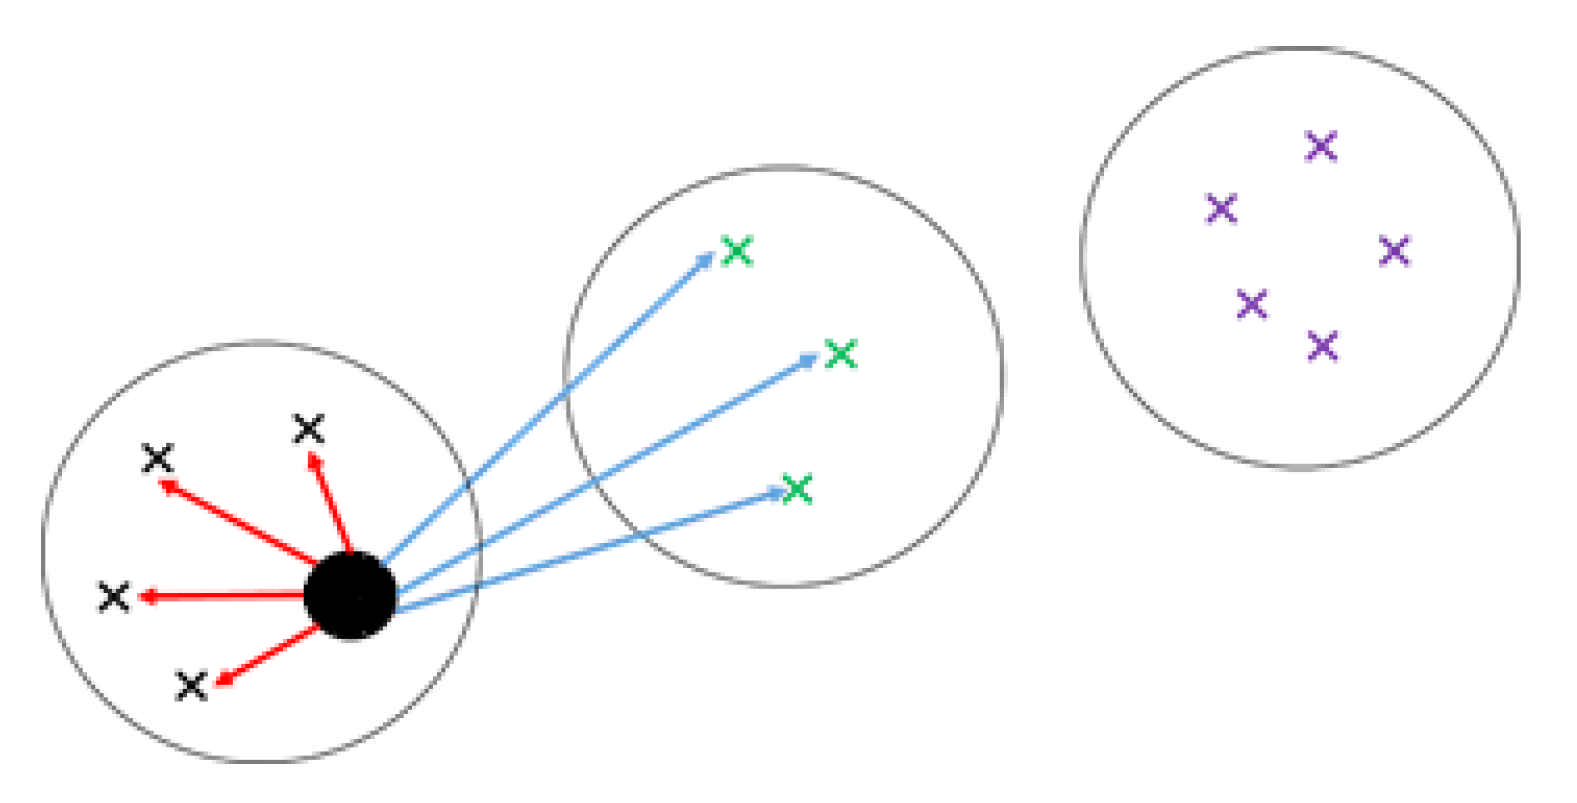
\includegraphics[width=.7\textwidth]{images/papers/silhouette_index.png}
			\caption{Visualization of silhouette index calculation~\cite{shutaywi2021silhouette}.  \label{fig:silhouette_index}}
		\end{figure}
	
The Silhouette index formula is represented for the data point $x_i$ (highlighted in dark) in ~\prettyref{fig:silhouette_index}, where the red lines represent the intra-cluster distances $a(x_i)$ and the blue lines represent the inter-cluster distances to the nearest cluster $b(x_i)$. In the best-case scenario, the value of $a(x_i)$ is very low compared to the value of $b(x_i)$, which results in well-formed clusters. Therefore, the goal of achieving heterogeneity can be measured using the silhouette score.

	
		\subsection{Extrinsic Evaluation:} To evaluate the quality of clustering with the help of document labels in the test set, a custom target function $F$ is designed. The target function $F$ tests the quality of clusters against the relevance labels from the dataset. The objective is to determine whether relevant documents are clustered into a similar cluster and the same applies to irrelevant documents. Without any relationship between clustering and relevance labeling, it cannot be assumed that positive and negative documents are automatically clustered together, as they may cover a wide range of keywords in different domains. Therefore, it is more meaningful to evaluate the clustering for negative documents, i.e., irrelevant and wrongly labeled documents. A target function is designed to address the number of negative documents isolated through sub-topic modeling.
		
		
The output of the sub-topic modeling pipeline is distinctive clusters with a unique context, independent of relevance to the user's intention. However, the clusters can be divided into relevant and irrelevant clusters based on the relevance labels in the dataset. Let us consider that $N_1, N_2, N_3, N_4$ represent functions to obtain the number of documents in a single cluster with label IDs $1, 2, 3, 4$ respectively, as shown in \prettyref{tab:label_definitions}, and $C$ represents the cluster set.
		
		\centerline{$C$ = $\{c_1, c_2, c_2,\dots\}$}
		
		Relevant clusters $C_r$ are clusters, that contain at least one document with label-id $1$ or documents with majority of label-id $2$. This can be determined using the below expression.
		
		\centerline{$C_r$ = $\{c_i \in C | (N_1(c_i) > 0) \lor (2 * N_2(c_i) >= (N_3(c_i) + N_4(c_i))) $}
		
		With this expression, relevant clusters are differentiated from others and the focus is only on labels $1$ and $2$. The clusters that do not satisfy the above condition are logically considered irrelevant clusters. 
		
		\centerline{$C_i$ = $\{c_j \in C \setminus C_r\} $}
		
The target function evaluates the clustering by calculating the ratio of irrelevant documents to the documents in the candidate pool $CP_q$ for a given user query $q$. For a total of $N$ queries, the target function maps the score using the equation below. The function $F$ ranges from 0 to 100, where a higher score indicates better separation of negative documents from positive documents, indirectly representing the diversity of clustering results.

		
		\centerline{$F$ = $\sum\limits_{i=1}^N (|C_i|/|CP_i|) * 100 $}
		
		\subsection{Objective Function:} Both the target functions \textit{Silhouette index} and $F$ are used to tune the parameters of the sub-topic modeling pipeline. The \textit{Silhouette index} evaluates the clustering output, and the custom target function $F$ evaluates the distribution of relevant labels. In order to perform automatic parameter selection, an objective function $O$ is proposed, which takes the harmonic mean of silhouette and target function scores. Since the scores are on different scales, both are normalized to a range [0-1] using min-max normalization. Therefore, $O$ ranges from [0-1], and the clustering parameters that generate a higher score are considered as the final sub-topic pipeline parameters. \prettyref{tab:hyper_parameters} shows the parameters that will be tested during clustering evaluation.\\
		
		\centerline{$O$ = $ \frac{(2 * S * F)}{(S + F)} $}
		
		\mycomment{An automatic parameter tuning can lead to very small clusters and there is a possibility of documents being marked as noise. Therefore,  A manual evaluation of these two metrics will be considered to finalize the pipeline parameters. }
		
		\subsection{Hyperparameter Selection:}
		
Three main components in the sub-topic modeling pipeline are candidate keyword selection, dimensionality reduction with \ac{UMAP}, and clustering using \ac{HDBSCAN}. Candidate keyword selection has only one parameter ranging from 10 to 100, signifying the percentile selection according to the query similarity. \ac{UMAP} dimensionality reduction has many parameters, but only the output data's reduced dimensions are considered for parameter selection. The other parameters are chosen after some preliminary tests. Two main parameters used in \ac{HDBSCAN} clustering are minimum cluster size and minimum samples. The minimum cluster size is a crucial parameter that determines the final cluster size of the clusters and is used by \ac{HDBSCAN} to merge clusters until the specified clustering size is achieved. Minimum samples signify the minimum number of neighbors to a core point. The larger the value of this parameter, the resulting clusters are denser, and more data points are labeled as noise points~\cite{hdbscanParameterSelection}. \prettyref{tab:hyper_parameters} shows the parameters used for clustering evaluation.

		
		
		\begin{center}
			\captionof{table}{Parameters used in the pipeline for testing.}\label{tab:hyper_parameters}
			\begin{tabularx}{.9\textwidth}{|c|Y|Y|}
				\hline
				S No. & Hyperparameters & Range  \\
				\hline
				1 & Candidate keyword selection parameter & [10, 15, 20, 25, 30, 35, 40, 45, 50, 55, 60, 65, 70, 75, 80, 85, 90, 95, 100]  \\
				\hline
				2 & Reduced dimensions (\ac{UMAP}) & [5, 10]  \\
				\hline
				3 & Min cluster size (\ac{HDBSCAN}) & [20, 25, 30, 35, 40, 45, 50, 55, 60 ]  \\
				\hline
				4 & Min samples (\ac{HDBSCAN}) & [1, 3, 5, 7, 10 ] \\
				\hline
			\end{tabularx}
		\end{center}
	  



\section{Survey Evaluation}

The sub-topics are assumed to help the user by retrieving the documents that are related to the query and sub-topics. This can be referred to as the assumption of user satisfaction. Precision analysis can evaluate this assumption when we have a dataset with two inputs rather than one input. Two inputs here denote the original query and an additional sub-topic. As \ac{FKIE} is keenly interested in specific topics of technology and the military, and the user intention is also restricted to the innovation-related theme, a manual evaluation with the help of a survey is chosen.



Two \ac{IR} systems, namely \textit{System A} and \textit{System B}, are designed to represent the documents during retrieval when a query and sub-topic are provided. This survey evaluates the performance of these two \ac{IR} systems. Template queries are used to retrieve and rank the text documents semantically. A template "Innovation in \textbf{Query} and \textbf{Sub-topic}" is used in the retrieval. The "Query" and "Sub-topic" are used as placeholders in the template and are dynamically replaced by actual values the user gives. In addition to evaluating the system, the sub-topic modeling output is also tested by taking the user's feedback on the quality of the sub-topics. Below are the two \ac{IR} systems developed and tested in the survey.


\begin{enumerate}
	\item 	\textbf{System A} is an \ac{IR} system that retrieves documents from the sub-topic cluster chosen by the user and re-ranks the retrieved documents using template similarity. Cosine similarity is used as the ranking function. \prettyref{fig:systemA} shows the pipeline to extract documents with system A.
	
	
\begin{figure}[h]
	\centering
	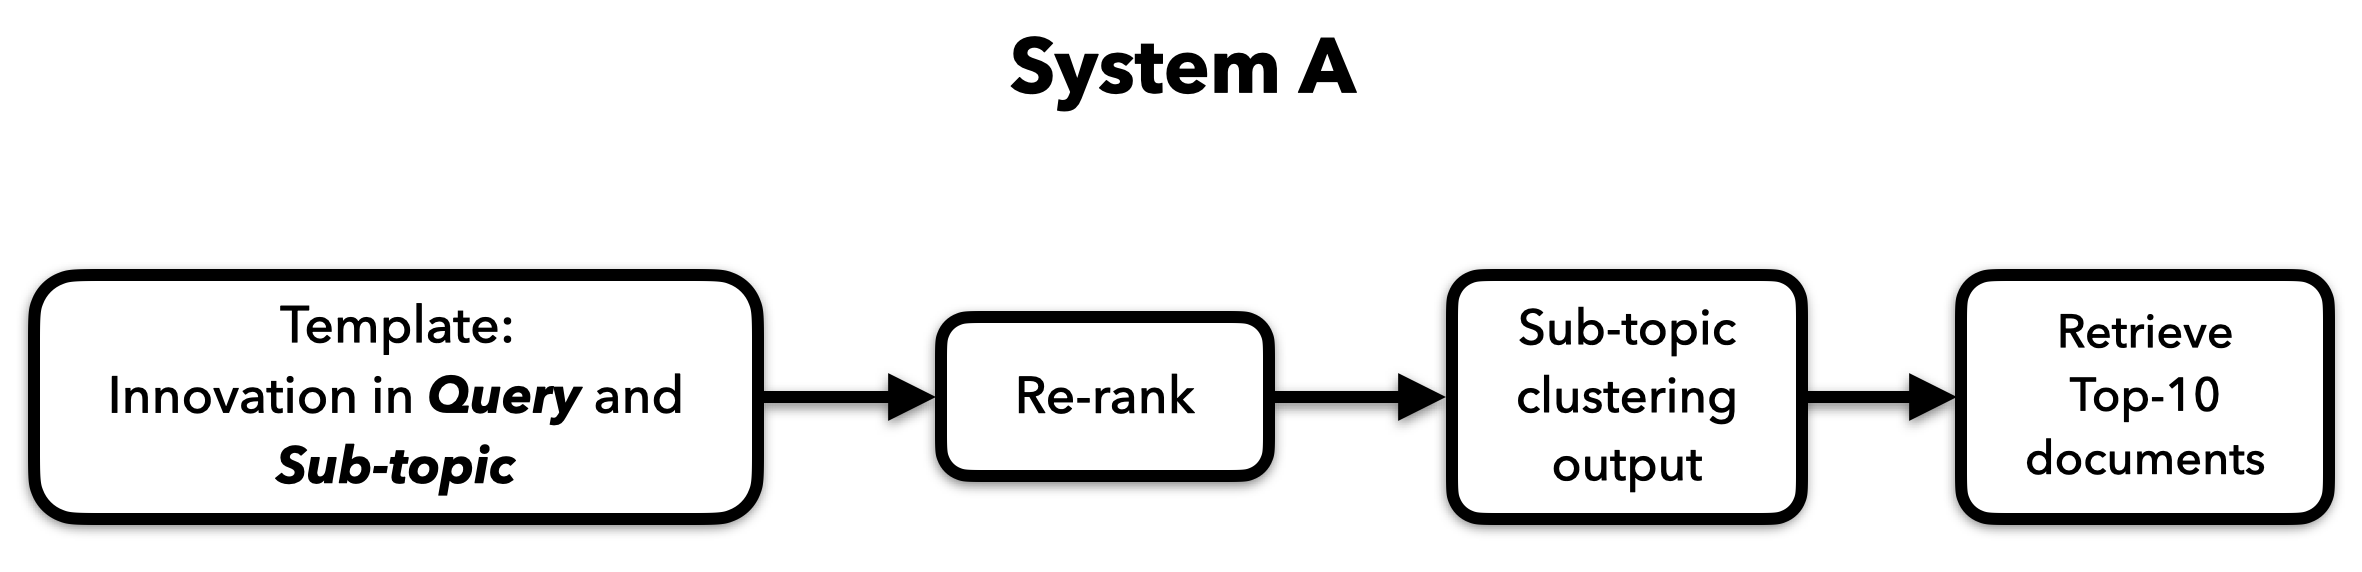
\includegraphics[width=.9\textwidth]{images/thesis_images/systemA.png}
		\caption{Steps to retrieve system A results. \label{fig:systemA}}
\end{figure}
	
	\item 	\textbf{System B} is an \ac{IR} system that retrieves documents semantically using a new search query generated by the template. As the documents are retrieved semantically, there is no need to re-rank the documents again. \prettyref{fig:systemB} shows the pipeline to extract documents with system B.
	
	
	\begin{figure}[h]
		\centering
		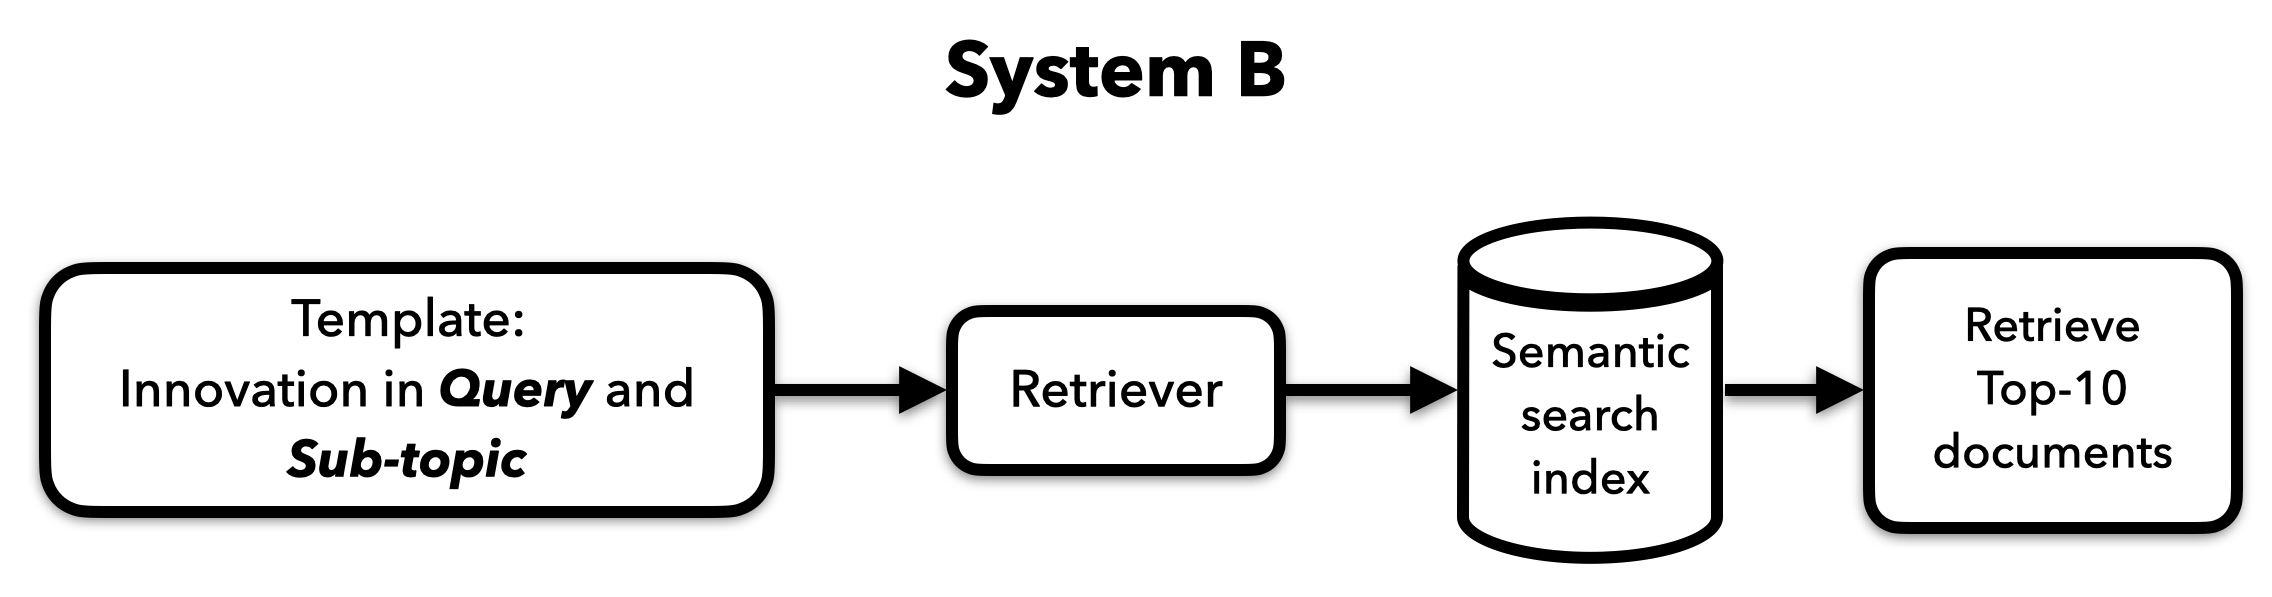
\includegraphics[width=.9\textwidth]{images/thesis_images/systemB.png}
		\caption{Steps to retrieve system B results. \label{fig:systemB}}
	\end{figure}
	
\end{enumerate}

\subsection{Survey questionnaire}

A website is developed to conduct the survey and collect participant data. The feedback collected is stored in an SQLite-DB. The participants of this survey are employees at \ac{FKIE}. The participants are invited through an email (not chosen by any particular means), and no personal user information is collected during the survey. Only a \ac{UUID} is used to differentiate users when filling out the survey concurrently. The user interface is developed in Python, FastAPI, Bootstrap, \ac{HTML}, and \ac{JS}, and deployed using Docker on the \ac{VM}. The code developed for the survey questionnaire is shared in a GitHub repository \textit{Survey-thesis}\footnote{\url{https://github.com/praveengadiyaram369/Survey-thesis}}.


\begin{figure}[h]
	\centering
	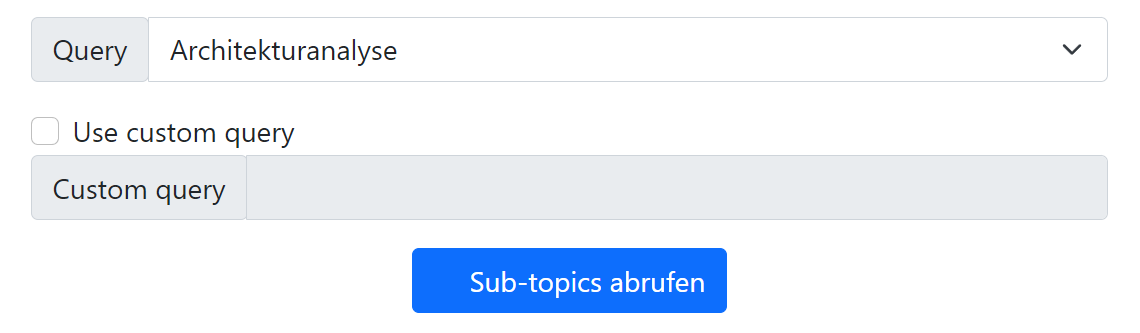
\includegraphics[width=.8\textwidth]{images/survey/query_input.png}
	\caption[Query input from the user.]{Survey UI showing query input either from the dropdown menu or a custom input. \label{fig:survey_question_1}}
\end{figure}

Five questions are developed to evaluate user satisfaction with the retrieved results and sub-topic modeling output. Survey participants are requested to provide a query either by selecting a query from the drop-down list or entering custom text through a text box. ~\prettyref{fig:sub_topic_output} depicts the user interface where participants provide the query. The queries provided in the drop-down list are restricted to a specific keyword list that is of interest for \ac{FKIE}. The keyword list contains queries in both English and German languages, and all participants see the same list. The query keywords list used in the survey is shared below.



\begin{description}
	
	\item [Query keywords list (in english and german)] \hfill \\ Architekturanalyse, Cloud Computing, Combat Cloud, Cyber-Verteidigung, Data Centric Warfare, Edge computing, Geoinformationen, IT-Bedrohungsanalyse, Interoperabilität, Kommunikationstechnologien, Kryptographie, Künstliche Intelligenz, Main Ground Combat System (MGCS), Mixed Reality, Mobile Kommunikation, Multirobotereinsatz, Prozessunterstützung, Quantentechnologie, Robotik, Satellitenkommunikation, Schutz von unbemannten Systemen, Semantische Technologien, Sensordatenfusion, Software Defined Networking, Taktische Datenlinks, Taktisches Routing, Unbemannte Landsysteme, Wellenformen und -ausbreitung
	
	
\end{description}

Subsequently, the sub-topics are retrieved during runtime and displayed to the user as a list. \prettyref{fig:sub_topic_output} shows the extracted sub-topic list for the query "Architekturanalyse". Participants are now asked to share feedback on the quality of this sub-topic list.


Following the feedback, participants are requested to select a sub-topic and retrieve documents relevant to the query and the sub-topic.  \prettyref{fig:survey_question_2} shows the retrieved \ac{IR} system results for the query "Architekturanalyse" and the sub-topic "Mikroprozessor". Once again, the participants are asked to share feedback on the system results by rating the systems quantitatively. Lastly, the participants are given an optional question regarding the significance of the whole sub-topic approach. The questionnaire used in the survey is briefly described below.


\begin{enumerate}
	\item ~\textbf{Is the above sub-topic clustering output distinctive and well-labeled?} \\
	
This question aims to evaluate the effectiveness of the approach proposed in the master thesis, i.e., well-formed heterogeneous clusters. Participants are requested to share feedback on the clustering output based on two characteristics, namely the distinctiveness and readability of the sub-topics. \prettyref{fig:sub_topic_output} shares the sub-topic clustering output for the query "Architekturanalyse". Distinctiveness describes the diversity of sub-topics, and readability depicts the ease of understanding the sub-topic by its name or label. The definitions of the labels are not explicitly provided to the participants as they are self-understanding. Below are the options provided to the survey participants, and only one option must be selected.

	
	\begin{enumerate}
		\item Distinctive and well-labeled
		\item Distinctive and not well-labeled
		\item Not distinctive and well-labeled
		\item Not distinctive and not well-labeled
	\end{enumerate}
	
	
	\begin{figure}[h]
		\centering
		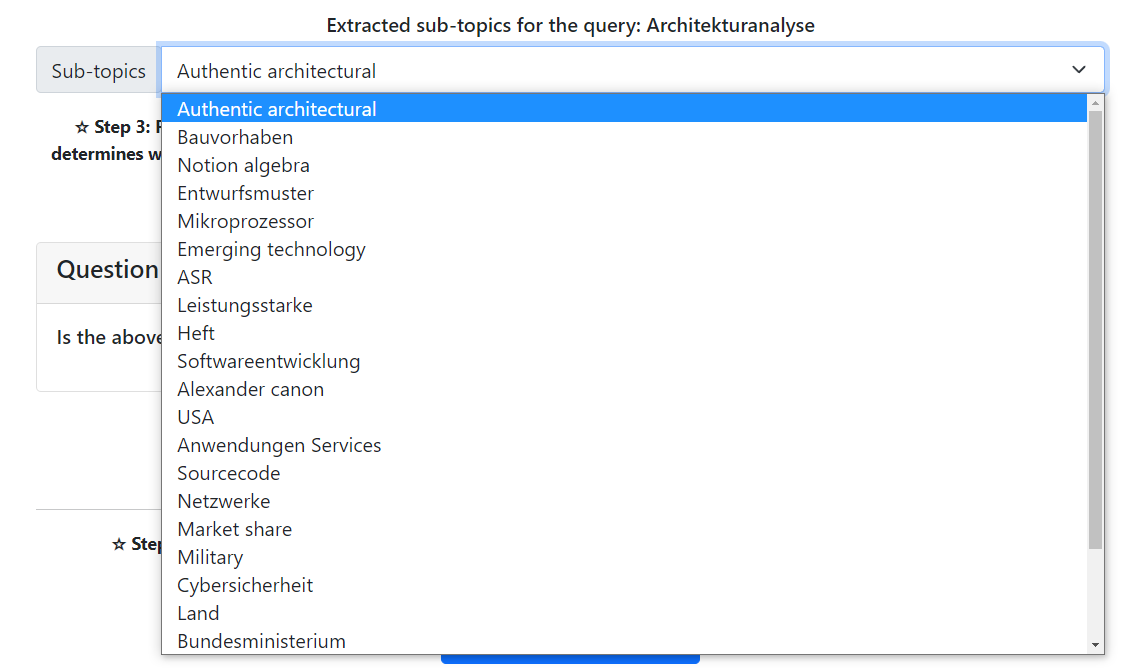
\includegraphics[width=.8\textwidth]{images/survey/sub-topic-output.png}
		\caption[Sub-topic list example.]{Extracted sub-topic list for the given query "Architekturanalyse". \label{fig:sub_topic_output}}
	\end{figure}
	
	
	\item ~\textbf{Which system results better represent the relevant news articles according to the given query and sub-topic?}  \\
	
Relevant news articles are retrieved text documents that have positive document characteristics (mentioned in Section 6.2). Participants are asked to read the retrieved results from \ac{IR} systems A and B and then share the feedback accordingly. \prettyref{fig:survey_question_2} shows the user interface with the system results. Below are the options provided to the survey participants, and only one option must be selected.

	
	\begin{enumerate}
		\item System A
		\item System B
		\item Neither System A nor System B
	\end{enumerate}
	
	\begin{figure}[h]
		\centering
		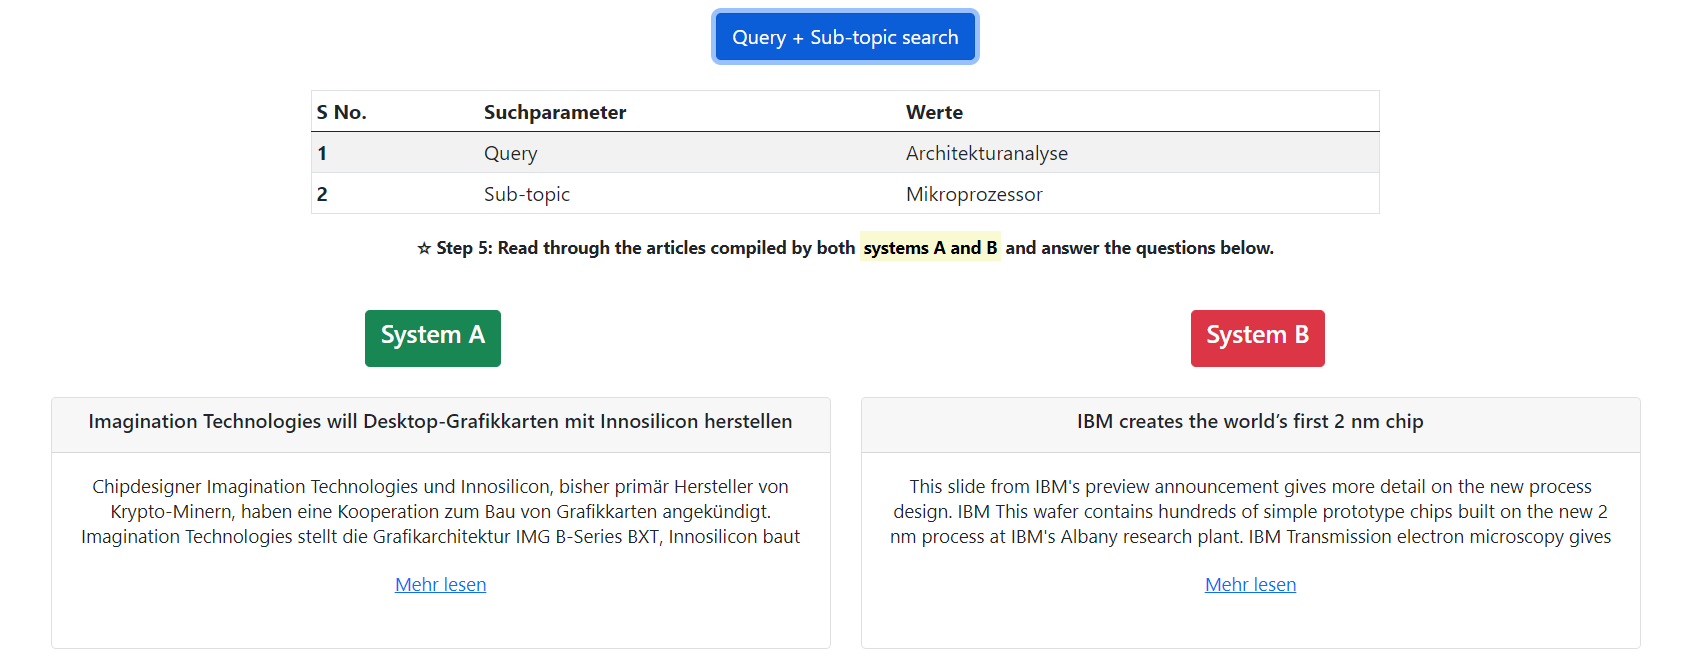
\includegraphics[width=.9\textwidth]{images/survey/sub-topic-search-output.png}
		\caption[Extracted \ac{IR} system results.]{Extracted \ac{IR} system results for a given user query and sub-topic. \label{fig:survey_question_2}}
	\end{figure}
	
	\item ~\textbf{Rate the retrieval system A results for the given query and sub-topic (0-10).} \\
	
Participants are requested to share quantitative feedback by rating the system's results A on a scale of 0 to 10. Ratings can include fractional values up to 1 decimal place. For example, a user can provide a rating of 3.4 but not 4.65. The user ratings directly indicate the user satisfaction corresponding to the retrieved results.

	
	\item ~\textbf{Rate the retrieval system B results for the given query and sub-topic (0-10).} \\
	
	Participants are requested to share a quantitative feedback by rating the system B results between 0 to 10.
	
	\item ~\textbf{Were the sub-topics helpful for you to find the relevant documents?} \\
	
This question aims to evaluate the usefulness of sub-topic modeling in \ac{IR}. It answers the practicality of using the proposed methodology in this master's thesis in a real environment to find innovation-related documents. Participants are requested to provide a boolean response of either "Yes" or "No" corresponding to whether it fulfills their expectations.

	
	\begin{enumerate}
		\item Yes
		\item No
	\end{enumerate}
	
\end{enumerate}

\section{Precision evaluation}

Assuming that the cluster labels could be more helpful to the user, the next evaluation technique shows that the clustering output does not deteriorate the performance of the retrieval results. The clustering output is difficult to examine with the baseline \ac{IR} systems because the order of documents needs to be included, and the performance metrics related to false positives need to be addressed. For this purpose, we are extending the sub-topic creation with sub-topic ranking and document ranking. These two rankings help the existing pipeline to create a sequential order of documents and facilitate the evaluation of precision against the baselines. Therefore, this evaluation approach proposes eight different retrieval systems and evaluates the ranked results.


\begin{center}
	\captionof{table}{Proposed \ac{IR} systems for evaluation.}\label{tab:ir_systems}
	\begin{tabularx}{0.8\textwidth}{|c|c|Y|}
		\hline
		 IR system name & Sub-topic ranking & Document ranking \\
		\hline
		 IR0 & NA & Uniform distribution \\
		\hline
		 IR1 & NA & Query similarity \\
		\hline
		 IR2 & Query similarity & Query similarity \\
		\hline
		 IR3 & Template similarity & Template similarity \\
		\hline
		 IR4 & Document cardinality & Query similarity \\
		\hline
		 IR5 & (IR4, IR2) & Query similarity \\
		\hline
		 IR6 & (IR4, IR2, IR3) & Query similarity \\
		\hline
		 IR7 & Random combinations & Query similarity \\
		\hline
	\end{tabularx}
\end{center}

The first system, \textit{IR0}, is an arbitrary system where the positive documents are uniformly distributed in the ranking order. \textit{IR1} system is a simple query re-ranking of results based on cosine similarity between the query and documents. The systems \textit{IR2, IR3, IR4} are the results of sub-topic pipeline clustering, where the clusters are first ranked, and later the documents are re-ranked with certain criteria. These three systems simulate the user reading the results linearly or in a sequence. In \textit{IR2}, the sub-topic clusters are ranked by the cosine similarity between the query and the centroid vector of the cluster, and similarly for document ranking.


The system \textit{IR3} uses a template similarity criterion, where the similarity is calculated between a template and centroid vector rather than the query. For example, the template string can be "Innovation and Technology". Similarly, \textit{IR4} clusters are ranked using the number of documents in the cluster. The last system, \textit{IR7}, is an unreal system just like \textit{IR0}, but multiple combinations of random rankings of clusters are considered to simulate the random selection of a sub-topic by the user and reading the documents in different sub-topics.


\subsection{Combinational IR systems}

The systems \textit{IR5} and \textit{IR6} are produced by combining sub-topic rankings of other \ac{IR} systems. The sub-topics are combined in such a way that the top-ranking sub-topics are clustered together. This approach adopts the benefits of two ranking criteria into a ranking. As a part of the exploratory analysis, the potential of sub-topic ranking is explored with these combinations. Algorithm \prettyref{algo:combined_ir} details the steps to generate a unique combined ranking output in the case of two individual rankings.


	\begin{algorithm}[H]
	\SetKwInput{KwInput}{Input}                % Set the Input
	\SetKwInput{KwOutput}{Output}              % set the Output
	\DontPrintSemicolon
	
	\KwInput{ranking\_lists - list $[ranking\_lists\_i]$, $i=1, 2, \cdots, n$, where each element is an individual ranking list }
	\KwOutput{combined\_ranking\_list - list $[combined\_ranking\_list\_i]$, $i=1, 2, \cdots, n$, where each element is a string }
	% \KwData{Testing set $x$}
	
	% Set Function Names
	\SetKwFunction{FRemovdup}{Combine\_individual\_ranking}
	
	% Write Function with word ``Function''
	\SetKwProg{Fn}{Function}{:}{}
	\Fn{\FRemovdup{$ranking\_list$}}{
			
		\;
		combined\_ranking\_list = []\;
		ranking\_list\_1 = ranking\_list[0]\;
		ranking\_list\_2 = ranking\_list[1]\;
		
		ranking\_list\_len = len(ranking\_list\_1)\;
		
		\;
		
		\For{$i\gets1$ \KwTo $ranking\_list\_len$}{
			
			\tcp{rank\_1 and rank\_2 signifies the ranking id of the sub-topics}
			
			rank\_1 = ranking\_list\_1 [$i$]\;
			rank\_2 = ranking\_list\_2 [$i$]\;
			\;

			\tcp{Append only if the rank id is not added to the combined ranking list}
			
			\If{rank\_1 not in combined\_ranking\_list}
			{
				combined\_ranking\_list.append(rank\_1))\;
			}
			\;
			
			
		   \If{rank\_2 not in combined\_ranking\_list}
			{
				combined\_ranking\_list.append(rank\_2))\;
			}
			\;
			
		}
		\;
		
		\KwRet combined\_ranking\_list\;
	}
	
	\caption{Generate combinational IR system.} \label{algo:combined_ir}
\end{algorithm}
 
The idea of ranking combinations is influenced by ensemble techniques in machine learning. Ensemble methods improve performance and create robust models by combining the strength of multiple weak-performing models \cite{bi2019machine}. This technique eliminates the individual model bias and consolidates the unique benefits of individual models. The output of combined \ac{IR} systems presents the opportunity to test a unique ranking of sub-topics. This unique ranking of sub-topics creates a unique sequential order of documents. Following Algorithm \prettyref{algo:combined_ir}, an example of the combined ranking output is presented in \prettyref{tab:ir5_result}.

 
 
 \begin{center}
 	\captionof{table}{Combined IR5 system results. }\label{tab:ir5_result}
 	\begin{tabularx}{0.8\textwidth}{|c|c|Y|}
 		\hline

 			IR system & Sub-topic ranking type & Ranking list of sub-topics \\
 		\hline
 		IR4 & Document cardinality  & [4, 3, 1, 2, 0] \\
 		\hline
 		IR2 & Query cardinality  & [1, 3, 0, 4, 2] \\
 		\hline
 		IR5 & (IR4, IR2) & [4, 1, 3, 0, 2] \\
 		\hline
 	\end{tabularx}
 \end{center}
 

\subsection{IR systems evaluation}

Mehlitz et al. \cite{mehlitz2007new} have introduced a new evaluation measure for \ac{IR} systems named the \textit{Expectation score}. The expectation score ($E$) is similar to Precision ($P$) but does not consider false positives. $E_k$ represents the number of positive documents at index $k$, whereas $P_k$ represents the ratio of positive documents at index $k$ to $k$. Similarly, the \textit{\ac{ME}} is proposed to analyze the mean number of positive documents for $N$ queries. This metric is especially useful for comparing \ac{IR} systems that retrieve the most relevant documents at a given index $k$.



\centerline{$ME@k$ = ($\sum\limits_{i=1}^N E_i@k) /N$}

Furthermore, Mean Average Precision (MAP) \cite{cormack2006statistical} is used to evaluate the ranking performance. MAP is calculated through the Average Precision (AP) metric, which is an average of precision scores only at the positive document indices. Let us consider that $G$ is a set of all positive document indices with size $g$. The average precision and mean average precision are formulated as below. MAP alone is sufficient to compare different \ac{IR} systems, and the system with the highest MAP value is considered the best \ac{IR} system.


\centerline{$AP$ = ($\sum\limits_{i=1}^G P_i) /g$}

\centerline{$MAP$ = ($\sum\limits_{i=1}^N AP_i) /N$}

\subsection{Literature Comparison}

Sub-topic retrieval has two crucial components, namely \textit{Sub-topic creation} and \textit{Document retrieval}. Sub-topic creation generates representations from large news articles for a given search query. Document retrieval deals with the extraction of ranked news articles for a given search query and sub-topic. In the end, the output of sub-topic retrieval is nothing but a ranked list of news articles. Therefore, the output of the proposed approach in this master thesis is compared with the literature work shared by Nogueira and Cho \cite{nogueira2019passage}. This retrieval approach from the literature is known as \textit{Passage Re-ranking with \ac{BERT}}, and it uses contextual representations from \ac{BERT} language models to retrieve and re-rank the text documents.



\textit{Passage Re-ranking} approach uses a \textit{Multi-stage ranking} architecture and is presented in Section 4.2 of Chapter 4. The compared literature has similar goals to the proposed approach, such as unsupervised, multi-lingual, contextual representations, and two-stage retrieval (for high recall). The literature uses \textit{Retriever} and \textit{Re-ranker} components, which retrieve candidate documents based on certain criteria and rank the retrieved documents, respectively. This approach was initially proposed for question-answering tasks. To generate candidate documents for a search query, three different techniques are employed, namely \textit{BM-25}, \textit{Bi-encoder retrieval}, and \textit{Candidate pool extraction}.


\begin{figure}[h]
	\centering
	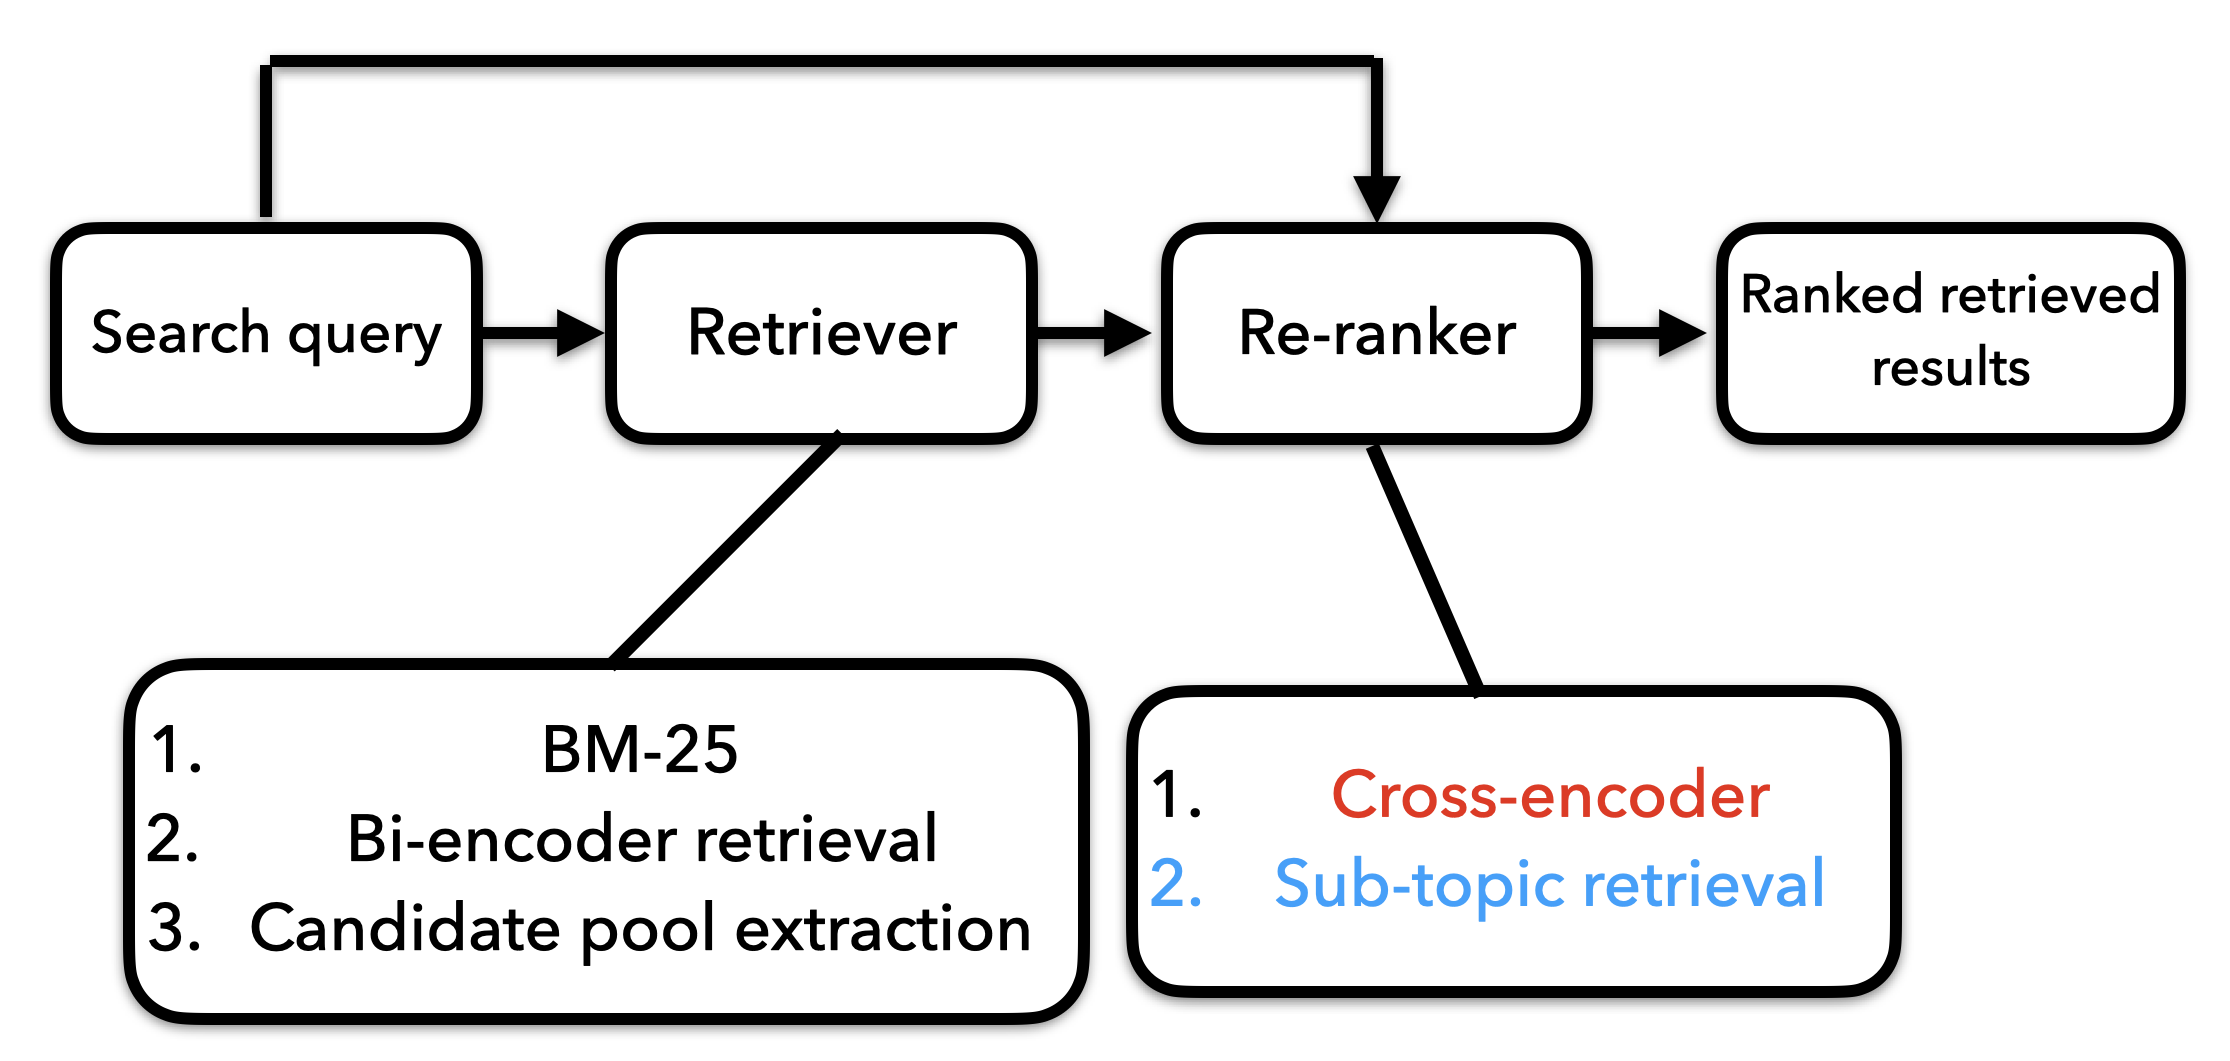
\includegraphics[width=.9\textwidth]{images/thesis_images/literature_review.png}
	\caption{Multi-stage ranking architecture. \label{fig:literature_review}}
\end{figure}

\begin{description}
	\item[BM-25]  \hfill \\ BM-25 is a probabilistic relevance algorithm which uses lexical matching approach to retrieve documents similar to the search query~\cite{amati_bm25_2009}
	
	\item[Bi-encoder retrieval]  \hfill \\ Bi-encoders are neural network models that encode the query and documents into dense vector representations. The encoded vector representations of the query and documents are then used to calculate the relevance similarity. The documents with higher query similarity are considered as retrieval output. A BERT-based multi-lingual bi-encoder model\footnote{\url{https://huggingface.co/LLukas22/all-MiniLM-L12-v2-embedding-all}} is used in this thesis to facilitate the extraction of candidate documents. The retrieved candidate documents using bi-encoder models are also referred to as the \textit{Semantic pool}.
	
	
	\item[Candidate pool extraction]  \hfill \\ Candidate pool extraction is an efficient retrieval method proposed in this master thesis to generate candidate documents for re-ranking. This approach considers both lexical and semantic matching approaches. More details about this approach are shared in Section 5.1 of Chapter 5.
	
\end{description}

Once the candidate news articles are extracted for a search query, the re-ranker ranks them based on query retrieval similarity. The ranking performance of two re-ranking approaches is evaluated using the \textit{Mean Average Precision} metric. The two approaches are namely \textit{Cross-encoder ranking} and \textit{Sub-topic retrieval}.



\begin{description}
	\item[Cross-encoder ranking]  \hfill \\ Cross-encoders are neural network models that encode the query and documents together and generate the relevance score between -1 and 1. The documents with higher query relevance similarity are considered as retrieval output. A BERT-based multilingual cross-encoder\footnote{\url{https://huggingface.co/amberoad/bert-multilingual-passage-reranking-msmarco}} model is used in this thesis to rank candidate documents generated from retrieval. The ranked results from the cross-encoder are compared to the proposed approach in the master thesis.
	
	
	\item[Sub-topic retrieval]  \hfill \\ The sub-topic retrieval output contains two ranking techniques to generate the final ranking of news articles. The first ranking technique is sub-topic cluster ranking, followed by document ranking. Eight different \ac{IR} systems with unique sub-topic and document rankings are proposed in Section 6.6, as shown in \prettyref{tab:ir_systems}. The system that performs the best is compared with the ranking output of the cross-encoder.
	
	
\end{description}


\section{Evaluation summarization}

The table \prettyref{tab:evaluation_rq} shares the evaluation techniques chosen in this master thesis and the respective research questions answered.

\begin{center}
	\captionof{table}{Proposed evaluation techniques. }\label{tab:evaluation_rq}
	\begin{tabularx}{0.9\textwidth}{|c|Y|Y|}
		\hline
 		S No. & Evaluation type & Research questions addressed \\
		\hline
		1 & Clustering analysis  & \textbf{RQ1} \\
		\hline
		2 & Survey questionnaire  & \textbf{RQ1, RQ2} \\
		\hline
		3 & Precision analysis and literature comparison & \textbf{RQ3} \\
		\hline
	\end{tabularx}
\end{center}




